\chapter{Аграрный вопрос}

Как же смешно наблюдать за свидетелями “России, которую мы потеряли”! Рассказывая о прекрасной России прошлого, они любят ссылаться на 1913 год с его красивой статистикой и "светлыми" перспективами. Для монархически настроенных граждан в той стране было и лучшее трудовое законодательство, и растущее в геометрической прогрессии благосостояние населения, и земельный вопрос у них решался. А я вот гляжу на это и задаюсь вопросом: как же в этой прекрасной стране могли случиться 3 революции?

Ответ-то на самом деле на поверхности лежит: Великие реформы Александра II при всём позитивном, что они принесли, вообще не сняли ключевых проблем государства. И самый яркий пример тут крестьянский вопрос. Аграрная реформа 1861 года должна была открыть сельское хозяйство для капитализма. Освобождение крестьян, наделение их землёй, переформирование помещичьих усадеб в современные хозяйства, стимулирование выхода крестьян из деревни в город — вот чего пытались добиться. Вот только добились чего-то не того.

Уже в 1861 году было очевидно, что с учётом роста крестьянского населения, наделов, достаточных для нормальной жизни, не хватит. Если честно поделить всю землю, то получится куча сверх-мелких и оттого неэффективных хозяйств. Выход, который придумали — а давайте пусть земля будет выдаваться общине. На бумаге всё гладко — коллективное землепользование же, на деле всё те же микронаделы. Так ведь мало этого — помещики перед этим нарезали себе самых сочных и нужных для хозяйственной деятельности земель, чтобы потом общинники вынуждены были её арендовать. Бизнес, понимаешь.

Но ладно, если бы это было единственной проблемой. Так ведь сам механизм реформы больше был похож на ограбление деревни, причём даже не помещиком, а самим государством. Логика-то была благородной: пусть крестьянин выплатит помещику 20\% выкупной суммы, а государство поможет с остальными 80\%. НО. Во-первых, эта сумма определялась, исходя из размера оброка, который мог вообще не быть привязан к реальной ценности земли. Во-вторых, крестьянин теперь должен был 80\% суммы государству, но есть нюанс: долг этот был, по сути, кредитом на 49 лет под 6\% годовых от общей суммы выкупного платежа. То есть, родное государство наваривалось на благом деле освобождения крестьян от гнёта, загоняя их в кабалу, но уже финансовую. По разным оценкам, к моменту отмены выкупных платежей в 1907 году, бюджет в общей сложности получил от них сверх других налогов и сборов с крестьян от 700 миллионов рублей до миллиарда. Почему не появились слухи, что царь и его министры тайные "жиды" — ума не приложу.

И ладно, если бы это всё имело какой-то высший смысл. Но нет. Помещики, получив деньги, тут же несли их иностранным банкирам, у которых были закредитованы чуть более, чем полностью . А всё, что осталось, можно было прокрутить в Монте-Карло и Баден-Бадене. Ни о какой организации хозяйств на современный лад речи не шло, так как эти процессы шли вовсе независимо. О каком-либо росте благосостояния крестьян и говорить не приходилось - какое благосостояние, когда царь-батюшка и клятые министры последние штаны снимают! Более того, не все могли вообще выкупить землю, и тогда для них не менялось вообще ничего: отрабатывай барщину или оброк, пока не сможешь расплатиться, милок. Не помогало переломить ситуацию ни снижение платежей, ни создание государственного ссудного банка для крестьян — государство выдаёт ссуду на получение от государства же ссуды. Это же гениальный развод лохов! Собственно, в 1907 году выкупную операцию отменили ввиду того, что многие долги по платежам были просто несобираемы — денег у крестьян не было, а потому те два года уже громили помещичьи усадьбы в крупнейшем крестьянском бунте, сопряженным с революцией в городах. Крестьянские восстания… в стране первого мира. Монархисты, вы не находите это странным?

Имперские экономисты, которые, согласно распространённому мифу, всё время думали "как бы нам запустить капитализм?", видимо, не додумались до простой истины: только платёжеспособный внутренний спрос на товары промышленности может стать драйвером её развития. А деревня как раз этого спроса и не формировала, от слова совсем. Огромное крестьянское население (за вычетом кулаков и наёмных работников ферм это будет от 50 до 60 \% на населения страны) будет долгие годы выключено из капиталистического хозяйства.

Систематическое ограбление деревни выкупными платежами, недостаток земли, отсталость хозяйства и невозможность, из-за вышеозначенных факторов, его модернизировать приведут к парадоксальной ситуации. Пока организованные по новым принципам крупные фермы стабильно повышали урожайность и, соответственно, валовый сбор урожая, деревня стагнировала и деградировала. Лишнее население деревни было некуда деть, так как слабая промышленность не могла всех впитать. А развиваться промышленности было некуда, так как спрос рос медленнее, чем она сама. Поэтому, несмотря на рост статки по сбору урожая, в 70-ые годы отрасль находилась в кризисе, который разразится в 80-ые из-за снижения цен на зерно. Крестьяне резко лишатся и так невеликих доходов от его продажи, а когда на это наложится неурожай – по стране прокатится голод. Сменить производственную культуру, что авторы современных книг по сабжу рекомендуют в такой ситуации, было нереально, так как зерно все равно выигрывало по урожайности и прибыльности даже после падения его цены. Совет же перейти на животноводство от тех же людей и вовсе смешон: для сохранения общей питательной ценности продукции для животноводства нужно в 3(!) раза больше земли, нежели для растениеводства, а земли нет.
\begin{figure}[h!tb] 
	\centering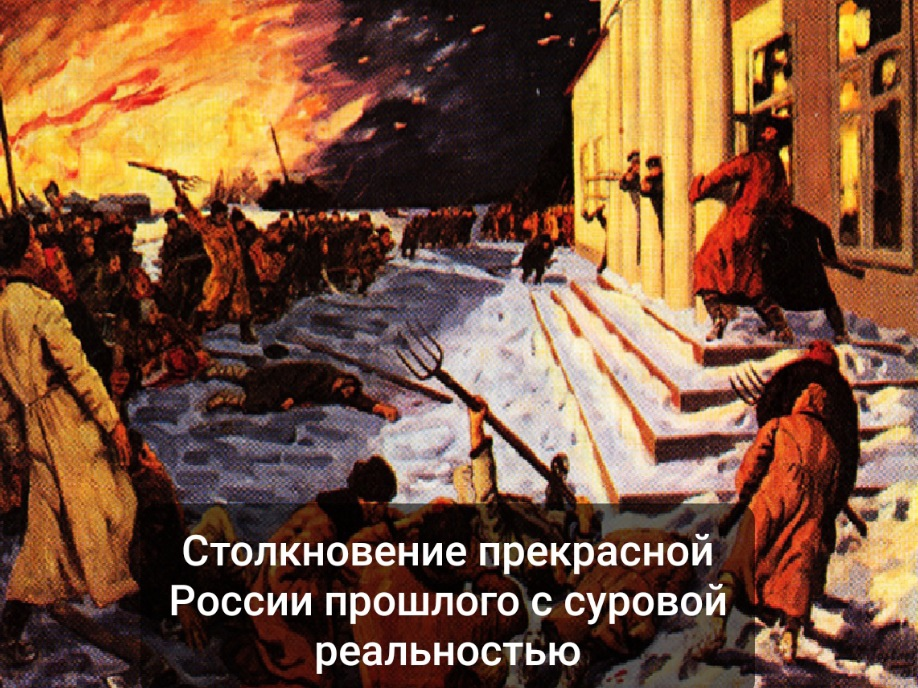
\includegraphics[scale=0.5]{Agrar_vopros/oPS7LqxV2xE.jpg}
	%	\label{fig:scipion} % Unique label used for referencing the figure in-text\end{document}
	%	%\addcontentsline{toc}{figure}{Figure \ref{fig:placeholder}} % Uncomment to add the figure to the table of contents%----------------------------------------------------------------------------------------
	%\caption{Если искать в интернете инфу про отца Морлиона, то найдется очень много различной литературы про знаменитых шпионов. Так или иначе, за Морлионом закрепилось звание агента ЦРУ — что, судя по найденной мною инфе, неудивительно. Я не очень в шпионских делах - может, когда-нибудь... }%	CHAPTER 2
\end{figure}
Точнее, она есть, но там, где никто жить не хочет. На этом факте и построил свою реформу Столыпин: мы вам деньги на переезд в незаселенные земли, а вы там стройте хозяйство, плодитесь и размножайтесь! Надо ли говорить, что когда после первых "успехов" до крестьян дошли слухи, что тебя просто высаживают в голом поле, никогда не возделываемом и где нет ничего, и на обустройство потребуется несколько лет, то желание ехать чёрте-куда поугасло. Не беда, сказали чиновники, и стали квадратно-гнездовыми методами насильно переселять людей, а потом пытаться решить проблему их бегства обратно. Не, ну а чё они, мы же для них и так всё сделали?! Ога. Всё это переселение сопровождалось классическим казнокрадством, воровством и отвратительным отношением чиновников к переселенцам. Надо ли говорить, что лишь единицы переселенцев построили крупные фермерские хозяйства, способные создать спрос на промышленные товары. В семье крепких кулаков в Северном Казахстане, из которой происходила моя бабушка, на 12 человек было 4 пары валенок, 2 пары парадных сапог, 2 лошади и 2 коровы. И такое хозяйство считалось кулацким! Круто же! Не?

Выбраться из кризиса сельского хозяйства помог рост цен на зерно и рост угодий фермеров, а не устранение коренных причин его возникновения. Да, Российская империя достигла огромного экономического прогресса при столь запущенной экономической базе, но в этом и беда — крестьянин всего этого роста экономики не видел. Он видел лишь, как кулаки и буржуи скупают землю разорившихся общинников, как нанимают батраков на работы за гроши, а потом разъезжают на самодвижущемся чуде технике и плюют на интересы общинников. А он сам живёт в замкнутом круге вечного выживания, выхода из которого не заметно — впереди лишь тлен и страдание, так как ни увеличить надел, ни бросить все и уйти в город, где работу еще искать надо, не мог. Последней попыткой решить проблему наигуманнейшее и прогрессивное правительство Николая II предприняло в ходе войны, решив переделить часть земли в пользу крестьян, для чего нужна была сущая мелочь — объявить врагами государства несколько миллионов его же граждан, имевших немецкие корни. Надо ли говорить, что эта реформа тоже осталась незавершённой и ничего бы не решила.

Отсюда и та безраздельная ненависть к помещикам, кулакам и другим эксплуататорам деревни, которая приведёт к тому, что кроме революций в верхах на деревне в 1917 году начнётся своя революция. Кровавая, с наматывание кишок на вилы, распиливанием людей, убийствами детей и прочим. Крестьян просто всё достало. Пускай там в городах мутят свои прожекты реформ, коли они не понравятся этому глубинному крестьянскому государству, то прожектёры отправятся туда же, куда и помещики — на вилы. И отправляли, регулярно и с огоньком аж до 1922 года, вне зависимости от цвета и лозунгов.

Автор Владимр Герасименко. Ссылка на оригинал \url{https://vk.com/wall-162479647_208143}
\#Герасименко@catx2
\#Заметка@catx2
